\chapter{ミリ波観測解析手法}
\label{ch:mm_analysis}
% 解析のフローチャートについて解、全体の解析の流れをしめす
% その背景を述べる(NOスペクトルの強度が微弱であることを含める)
\ref{ch:mm_obs}章で述べたように、トロムソは我々にとっては観測自体がはじめての場所であり、昭和基地においては分光計を更新してからはじめての観測である。
そのため、それぞれ観測装置立ち上げ後に行われたテスト観測のデータを1つずつ精査した。
また、\ref{sec:mm_syowa}節の図\ref{fig:NO_spectr}で示したように\ce{NO}の輝線スペクトルはとても微弱である。
そのため、S/N比がよい状態で輝線スペクトルを抽出する必要がある。
今回、\ce{NO}の柱密度の導出をするにあたって、スクリーニング(特定の条件を設定し、全体のデータから解析に用いることができるデータのみを選別)と電波強度の補正を行った。
ミリ波分光に関する装置は市販されていないため観測装置は自作となっており、その関係でスクリーニング、電波強度の補正に関わるプログラムは自ら作成した。
スクリーニングと電波強度の補正については、以下のようにそれぞれ2つの観点から行った。
\begin{itemize}
    \item スクリーニング
    \begin{itemize}
        \item 光学的厚みデータを用いたスクリーニング(\ref{sec:screening_opticaldepth}節)
        \item NOスペクトルデータに含まれるノイズによるスクリーニング(\ref{sec:screening_spectralnoise}節)
    \end{itemize}
    \item 電波強度の補正
    \begin{itemize}
        \item 光学的厚みデータの補正(\ref{sec:correction_opticaldepth}節)
        \item NOスペクトルデータのベースラインの補正(\ref{sec:correction_baselinefitting}節)
    \end{itemize}
\end{itemize}
\ref{sec:screening_opticaldepth}節と\ref{sec:correction_baselinefitting}節までのスクリーニングを行った結果、解析期間についてトロムソでは2019年1月23日 - 2019年2月4日と2019年2月17日 - 2019年2月20日、南極・昭和基地では2023年3月22日 - 2023年3月30日となった。
\ref{ch:mm_analysis}節では、それぞれの手法について上記のように順番に述べていき、最後の\ref{sec:derive_columndensity}節では柱密度の導出手法について述べる。

\section{光学的厚みデータを用いたスクリーニング}
\label{sec:screening_opticaldepth}

\ref{sec:mm_obs}節で述べたように、ミリ波分光計を用いた地上観測では下層大気による影響を受けるため、光学的厚みの測定データを用いてこの影響を取り除く必要がある。
したがって、光学的厚みの測定データは観測データに対して充分に安定していなければならない。
図\ref{fig:optical_depth_tromsoe}に示しているデータは、トロムソの観測装置立ち上げ後行われたテスト観測に測定された光学的厚みの時間変化を表したものである。
\begin{figure}[htbp]
    \centering
    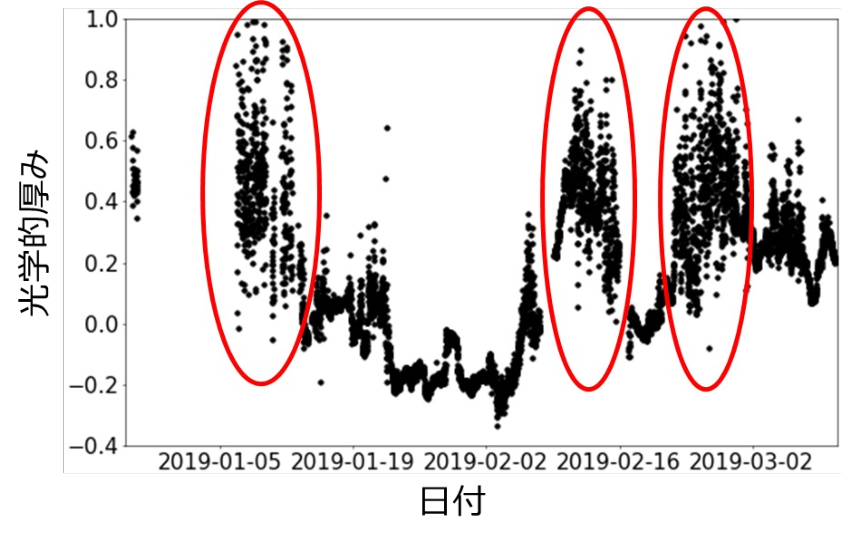
\includegraphics[width=\linewidth]{master_thesis_contents/master_thesis_fig/optical_depth_tromsoe.pdf}
    \caption{トロムソでの光学的厚み測定データの時間変化(~\cite{goto2021bachelor}より引用)}
    \label{fig:optical_depth_tromsoe}
\end{figure}
比較的値が安定している時期と、値が大きくばらついて安定していない時期がある(例として赤丸で示す)。
この赤丸で示された時期は、光学的厚みの典型値(たとえば南極昭和基地ではおよそ$0.1-0.4$の範囲の値をとる)とは大きく外れている。
さらに、このように短時間での値の変動が大きい場合は、それぞれ光学的厚みが測定された時間の間で下層大気の影響が一様でないことになる。
そのため、測定された光学的厚みの値を用いて、光学的厚みが測定された時間の間に観測された電波強度の補正をするには適さないと考えられる。
そこで、観測データの強度の補正に使用できる光学的厚みデータを判別するために、まず光学的厚みデータのスクリーニングを行うことを考える。
このスクリーニングで残った期間のNOスペクトルデータを後の解析に用いることとする。
判別方法としては、1日ごとにデータを区切りそれぞれの日の範囲で分散を計算し、その分散が$0.005$以下の値の日をとるデータを使用することとし、これを観測データのスクリーニングの条件として使用した。
この条件を設定することで、光学的厚みの変動が大きい日のデータを除去することができる。
分散の閾値を0.005としたのは図\ref{fig:optical_depth_tromsoe}のデータを目視し、値が安定していると判断した$2019年1月23日 - 2019年2月4日$の分散がいずれも0.005以下であったため、このように設定した~\cite{goto2021bachelor}。
南極・昭和基地の解析においても同条件でスクリーニングを行った。

\section{NOスペクトルデータに含まれるノイズによるスクリーニング}
\label{sec:screening_spectralnoise}

NOスペクトルデータにおいて、解析に使うことのできない質の悪いデータを事前にスクリーニングすることを考える。
トロムソの観測期間の全取得データを精査した結果、ノイズを含むスペクトルデータにおいて、スパイク状のノイズを含むデータと全体的にノイズを含むデータの2種類に大別できることがわかった~\cite{goto2021bachelor}。
スパイク状のノイズを含むデータと全体的にノイズを含むデータをそれぞれ判別する条件を考えることで、図\ref{fig:raw_spectrum}(a)のような質の良いデータのみを抽出することを目指す。
まず、NOスペクトルが存在する周波数を含むチャネル5000-10000の範囲のデータに対し2次曲線をフィッティングし、全体的にノイズがどれだけ含まれているか調べるために近似値に対する測定値の2乗平均誤差を計算した。
ここではチャネル5000-10000においてスペクトルデータの変動が二次関数的であったため、二次近似を用いている(図\ref{fig:raw_spectrum}(a)の赤線)。
\begin{figure}[htbp]
    \centering
    \begin{minipage}{0.33\linewidth}
        \centering
        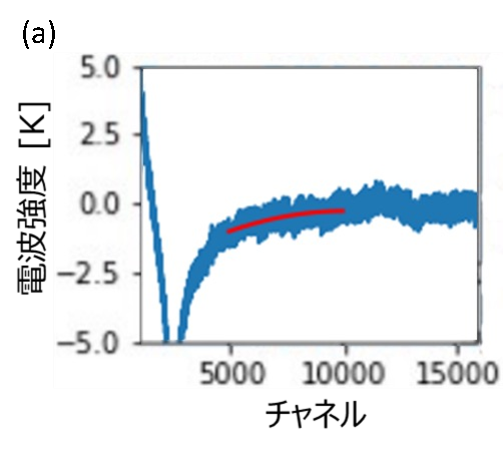
\includegraphics[width=\linewidth]{master_thesis_contents/master_thesis_fig/raw_spectrum_good.pdf}
        % \subcaption{解析に用いるために望ましい生データの一例($5000\, \mathrm{ch}$以下のデータは$239.093279\, \mathrm{GHz}$のオゾンの放射スペクトルデータがFRSWにより反映された結果、赤線は$5000-10000\, \mathrm{ch}$でのスペクトルデータの近似二次曲線を表す。~\cite{goto2021bachelor}より引用)}
        % \label{fig:raw_spectrum_good}
    \end{minipage}
    \begin{minipage}{0.6\linewidth}
        \centering
        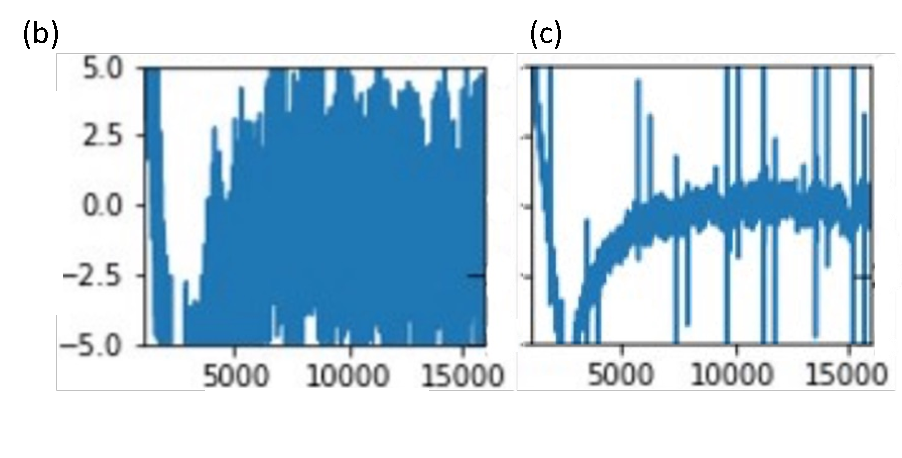
\includegraphics[scale=0.6]{master_thesis_contents/master_thesis_fig/raw_spectrum_bad.pdf}
        % \subcaption{スクリーニングしたいデータの例(左は全体的にノイズを含む例、右はスパイク状のノイズを含む例を表す)}
        % \label{fig:raw_spectrum_bad}
    \end{minipage}
    \caption{(a)解析に用いるために望ましい生データの一例($5000\, \mathrm{ch}$以下のデータは$239.093279\, \mathrm{GHz}$のオゾンの放射スペクトルデータがFRSWにより反映された結果、赤線は$5000-10000\, \mathrm{ch}$でのスペクトルデータの近似二次曲線を表す。)。(b)(c)スクリーニングしたいデータの例((b)は全体的にノイズを含む例、(c)はスパイク状のノイズを含む例を表す)。}
    \label{fig:raw_spectrum}
\end{figure}
これらの結果から、スクリーニング条件としては以下2つを設定した~\cite{goto2021bachelor}。
\begin{itemize}
    \item 2乗平均誤差の整数丸め値が0である
    \item チャネル5000-10000で強度の絶対値が$5\, \mathrm{K}$以上の値を含まない
\end{itemize}
1つ目の条件は、全体的にノイズを含むデータ(たとえば図\ref{fig:raw_spectrum}(b))を判別・除去することを意図しており、2つ目の条件はスパイク状のノイズを含むデータ(たとえば図\ref{fig:raw_spectrum}(c))を除去することを意図している。
設定したスクリーニング条件が妥当かどうかの検証は卒業研究~\cite{goto2021bachelor}にて行った。

\section{光学的厚みデータの補正(Troms\o)}
\label{sec:correction_opticaldepth}
\ref{sec:screening_opticaldepth}節の述べたように、不安定な光学的厚みのデータを除去するスクリーニングの結果によって、トロムソの観測データにおいて図\ref{fig:optical_depth_minus}のように期間A(2019年1月23日 - 2019年2月4日)、期間B(2019年2月17日 - 2019年2月20日)が残った。
しかし、期間Aにおいて光学的厚みが$-0.2$付近の負の値をとっていることがわかった(図\ref{fig:optical_depth_minus}の赤丸)。
\begin{figure}[htbp]
    \centering
    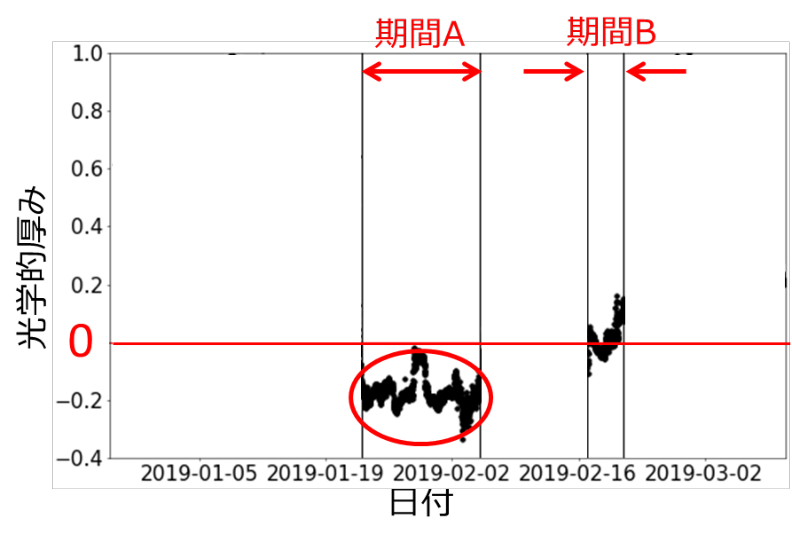
\includegraphics[width=\linewidth]{master_thesis_contents/master_thesis_fig/optical_depth_minus.pdf}
    \caption{トロムソにおいて負の値をとる光学的厚み(~\cite{goto2021bachelor}より引用)}
    \label{fig:optical_depth_minus}
\end{figure}
\ref{ch:mm_obs}章で述べた光学的厚みの算出方法のことを考えると、下層大気の光学的厚みの値が負の値を取ることはない。
そこでこの原因を調べたところ、光学的厚みを算出する際の各観測天頂角に対するプロットデータにおいて、もっとも観測天頂角が小さい($\sec z$が1番小さい)
ところのプロットデータが下に落ち込んでおり、それによって近似直線の傾きが変化してしまうことで、光学的厚みが負の値として計算されていることが分かった~\cite{goto2021bachelor}。
その模式図を図\ref{fig:optical_depth_slope_minus}、実際の測定データ例を図\ref{fig:optical_depth_measurement_good_bad}に示す。
\begin{figure}[htbp]
    \centering
    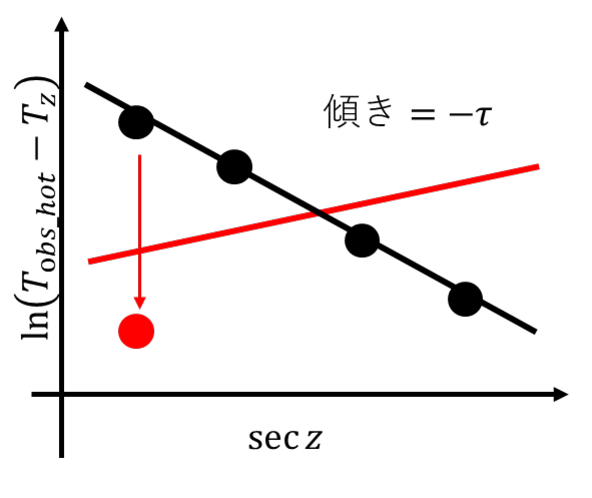
\includegraphics[width=\linewidth]{master_thesis_contents/master_thesis_fig/optical_depth_slope_minus.pdf}
    \caption{プロットデータの落ち込みによる光学的厚みの計算値の変化(プロットデータの落ち込みにより近似直線が黒線→赤線に変わり、直線の傾きが変わる)~\cite{goto2021bachelor}より引用。}
    \label{fig:optical_depth_slope_minus}
\end{figure}
\begin{figure}[htbp]
    \centering
    \begin{minipage}{0.41\linewidth}
        \centering
        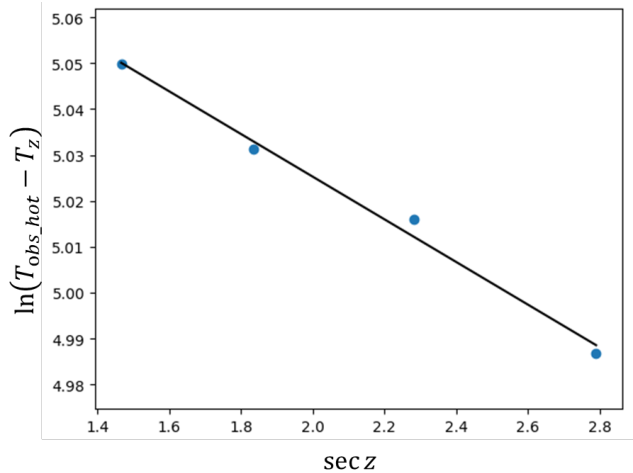
\includegraphics[width=\linewidth]{master_thesis_contents/master_thesis_fig/optical_depth_good.pdf}
    \end{minipage}
    \begin{minipage}{0.45\linewidth}
        \centering
        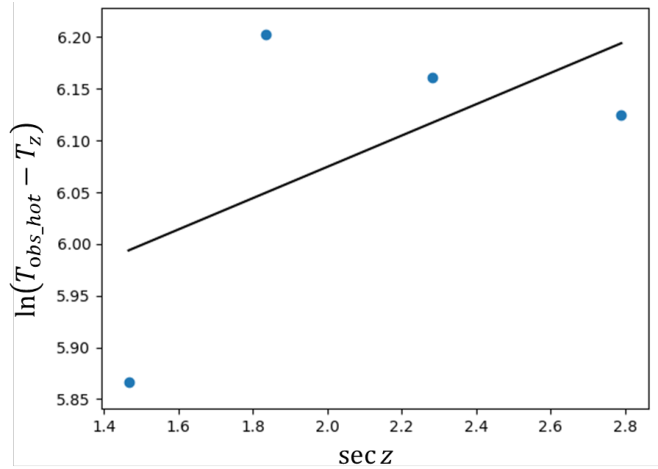
\includegraphics[scale=0.6]{master_thesis_contents/master_thesis_fig/optical_depth_bad.pdf}
    \end{minipage}
    \caption{(a)望ましいプロットデータの一例(2019年2月17日5時51分頃測定)。(b)プロットデータが落ち込んだ実際のデータの一例。(2019年1月23日0時5分頃測定)。黒線は近似直線を表す。~\cite{goto2021bachelor}より引用。}
    \label{fig:optical_depth_measurement_good_bad}
\end{figure}
さらに、そのプロットデータの落ち込みの原因を調べたところ、ちょうど光学的厚みの値が負の値となっている期間の終わりごろに、ミリ波観測装置のビームが通る側面の観測窓の上部に氷柱ができているのを見つけたという報告があり(図\ref{fig:icicles})、それが時期的に一致していることが分かった~\cite{goto2021bachelor}。
\begin{figure}[htbp]
    \centering
    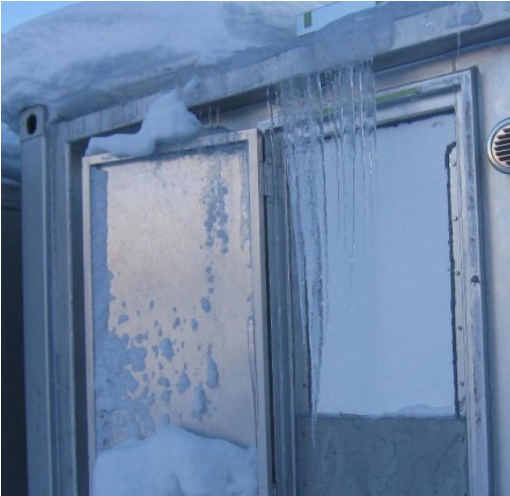
\includegraphics[width=\linewidth]{master_thesis_contents/master_thesis_fig/icicles.pdf}
    \caption{側窓にできた氷柱(~\cite{goto2021bachelor}より引用)}
    \label{fig:icicles}
\end{figure}
したがって、天頂角がもっとも小さい角度で測定された電波強度に影響を与えた可能性があると考え、そのデータを用いずに光学的厚みを測定し直し、光学的厚みの補正を行った。
設定した補正手法が妥当かどうかの検証は卒業研究~\cite{goto2021bachelor}にて行った。

\section{NOスペクトルデータのベースラインの補正}
\label{sec:correction_baselinefitting}
\ref{sec:screening_opticaldepth}節や\ref{sec:screening_spectralnoise}節によるスクリーニングで残った期間における\ce{NO}スペクトルデータについて積分を行う(積分時間はトロムソでは24時間、南極・昭和基地では12時間)。
これは昭和基地で行われた先行研究であるIsonoらによる研究~\cite{isono2014ground}より、1日程度の積分をすることで十分なS/N比で議論することができると考えたためである。
そして、観測データに含まれている\ce{NO}のスペクトルを検出するため、ベースラインの補正を行う。
ここでは、スペクトルの両端におけるデータを用いてバックグラウンドのベースラインを近似から求め、それを元のスペクトルから差し引くことによって、FRSWで除去しきれなかったオフセット成分や周波数特性のうねりなどをを除去した。
ベースラインの補正の模式図を図\ref{fig:baseline_correct_schema}に示す。
\begin{figure}[htbp]
    \centering
    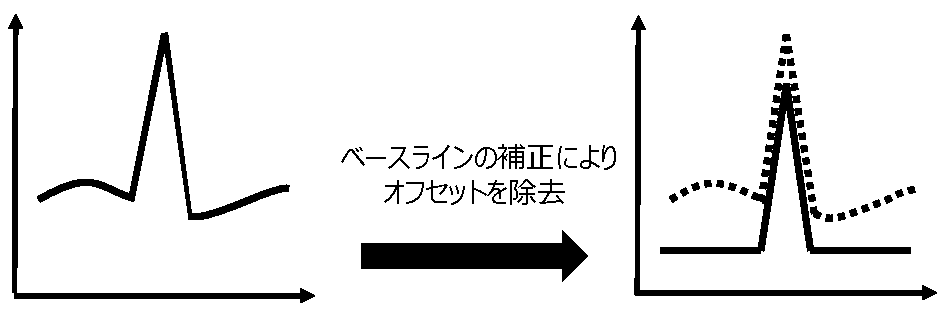
\includegraphics[width=\linewidth]{master_thesis_contents/master_thesis_fig/baseline_correct_schema.pdf}
    \caption{ベースライン近似を用いたベースラインの補正}
    \label{fig:baseline_correct_schema}
\end{figure}
ベースラインの近似に用いるデータは、図\ref{fig:baseline_range}の赤色で示したスペクトルの両端のそれぞれ$5\, \mathrm{MHz}$の範囲とした。
% 近似の範囲は、syowaだといくつ?
この範囲は、対象とするNOの放射スペクトル成分が含まれないと考えられる。
\begin{figure}[htbp]
    \centering
    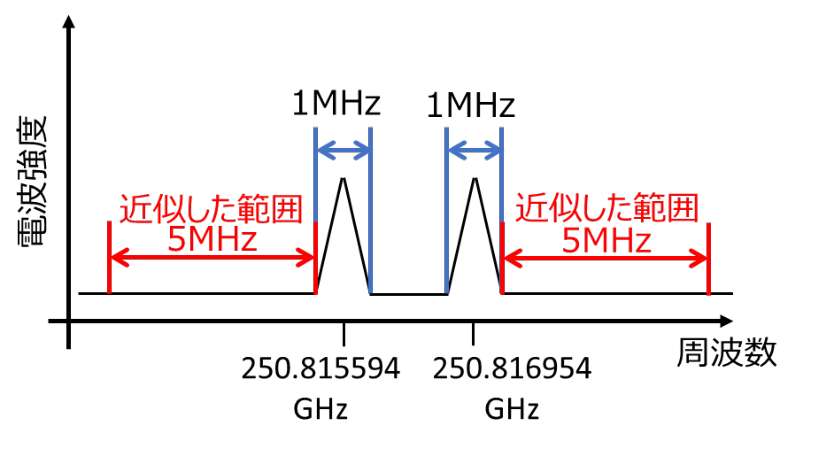
\includegraphics[width=\linewidth]{master_thesis_contents/master_thesis_fig/baseline_range.pdf}
    \caption{ベースラインを補正する元となる周波数の範囲(赤色で表示。青色は検出するスペクトルの幅を示している。例としてトロムソで用いた2本の輝線スペクトルの場合を示した。)}
    \label{fig:baseline_range}
\end{figure}
スペクトルデータのベースラインの特性の傾向が、図\ref{fig:baseline_curve}示す赤い曲線のような三次関数的な形であったので、ここでは三次関数で近似を行うことにした。
\begin{figure}[htbp]
    \centering
    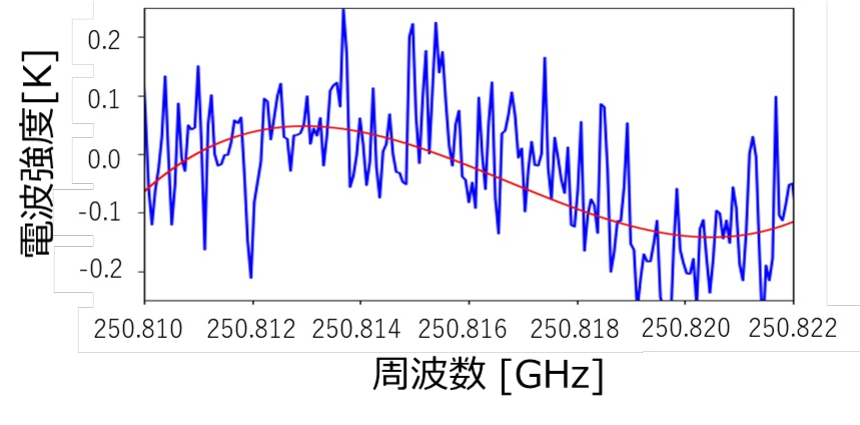
\includegraphics[width=\linewidth]{master_thesis_contents/master_thesis_fig/baseline_curve.pdf}
    \caption{三次関数的な形のベースライン(~\cite{goto2021bachelor}より引用)}
    \label{fig:baseline_curve}
\end{figure}
また、\ce{NO}の各スペクトル幅は$1\, \mathrm{MHz}$と仮定した。
このように仮定したのは対象の時期の日ごとのデータにおいて、放射スペクトルである三角の山状の幅の大きさがどの日のデータにおいてもおよそ$1\, \mathrm{MHz}$であることが確認できたためである(図\ref{fig:no_spectr_exp}にあるデータの一例において、スペクトル幅がおよそ$1\, \mathrm{MHz}$であることが確認できる)。
\begin{figure}[htbp]
    \centering
    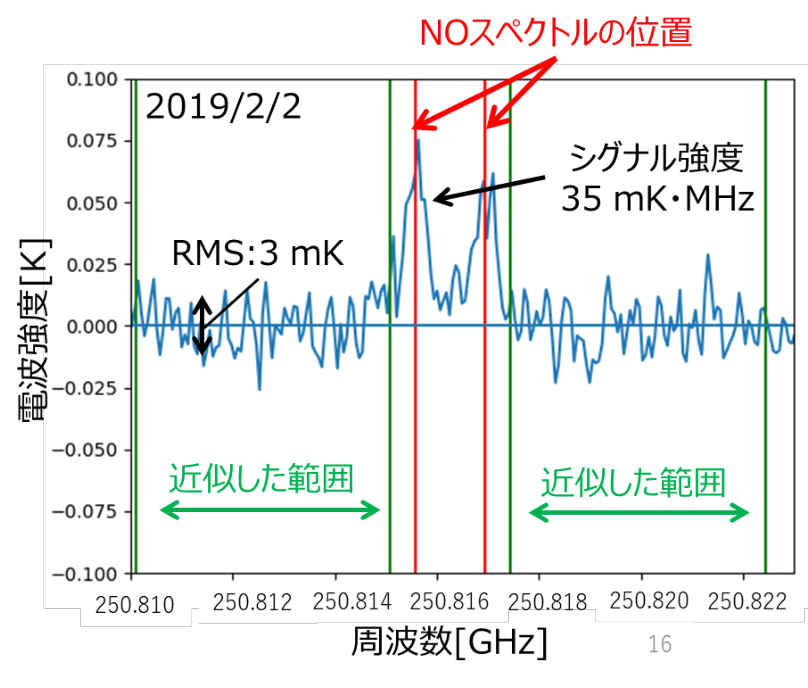
\includegraphics[width=\linewidth]{master_thesis_contents/master_thesis_fig/no_spectr_exp.pdf}
    \caption{スペクトルの検出の一例(赤線は検出するスペクトルがある周波数の位置、緑線はベースライン近似に用いたスペクトルデータの範囲を示す。~\cite{goto2021bachelor}より引用)}
    \label{fig:no_spectr_exp}
\end{figure}
\clearpage

\section{NO柱密度の導出}
\label{sec:derive_columndensity}
柱密度とは高度方向に密度を足し合わせたものであり、今回はスペクトルの線形から$70\, \mathrm{km}$以上に存在する\ce{NO}分子についてみたものとなる。
柱密度の導出においては先行研究~\cite{isono2014ground}を参考にして行った。
導出に用いた式は以下のようになる。
\begin{gather}
    N_{\mathrm{NO}} = A \times T_{\mathrm{atm}} \times \int T_{\mathrm{NO}}d\nu \\
    N_{\mathrm{NO}}:\ce{NO}の柱密度[\mathrm{cm^{-2}}]、A:線スペクトル強度係数[\mathrm{K^{-2}} \mathrm{MHz^{-1}} \mathrm{cm^{-2}}] \notag \\
    T_{\mathrm{atm}}:大気温度[\mathrm{K}]、\int T_{\mathrm{NO}}d\nu:\ce{NO}のスペクトル積分強度 \notag
\end{gather}
線スペクトル強度係数は輝線スペクトルの強度を知るための分子パラメーターで分子・周波数ごとに決まる値となる。
今回用いた\ce{NO}の輝線スペクトルにおけるそれぞれの線スペクトル強度係数については\ref{ch:mm_analysis}章の表\ref{tb:no_spectr_freq}に記載してある。
大気温度については一様に$200\, \mathrm{K}$と仮定し、\ce{NO}が存在する領域においては光学的に薄いと仮定している。
